\subsubsection{Versuch: Herstellung von PMMA}
\label{subsubsec:versuchpmma}

Material:
\begin{itemize*}
    \item Heizplatte, Reagenzgläser, Thermometer, Wasserbad, Spatel, Waage, Stativ
    \item Chemikalien: Methylmethacrylat (MMA; Sicherheitshinweis: CAS Nr. 80-62-1 (\autoref{fig:flamme}, \autoref{fig:ausrufezeichen})), Azodiisobutyronitril (AIBN; Sicherheitshinweis: CAS Nr. 80-62-1 (\autoref{fig:flamme}, \autoref{fig:ausrufezeichen})), Dibenzoylperoxid (BPO; Sicherheitshinweis: CAS Nr. 80-62-1 (\autoref{fig:flamme}, \autoref{fig:ausrufezeichen}, \autoref{fig:bombe}))
\end{itemize*}

\begin{figure}[h]
    \begin{center}
        \begin{minipage}[t]{0.25\textwidth}
            \begin{center}
                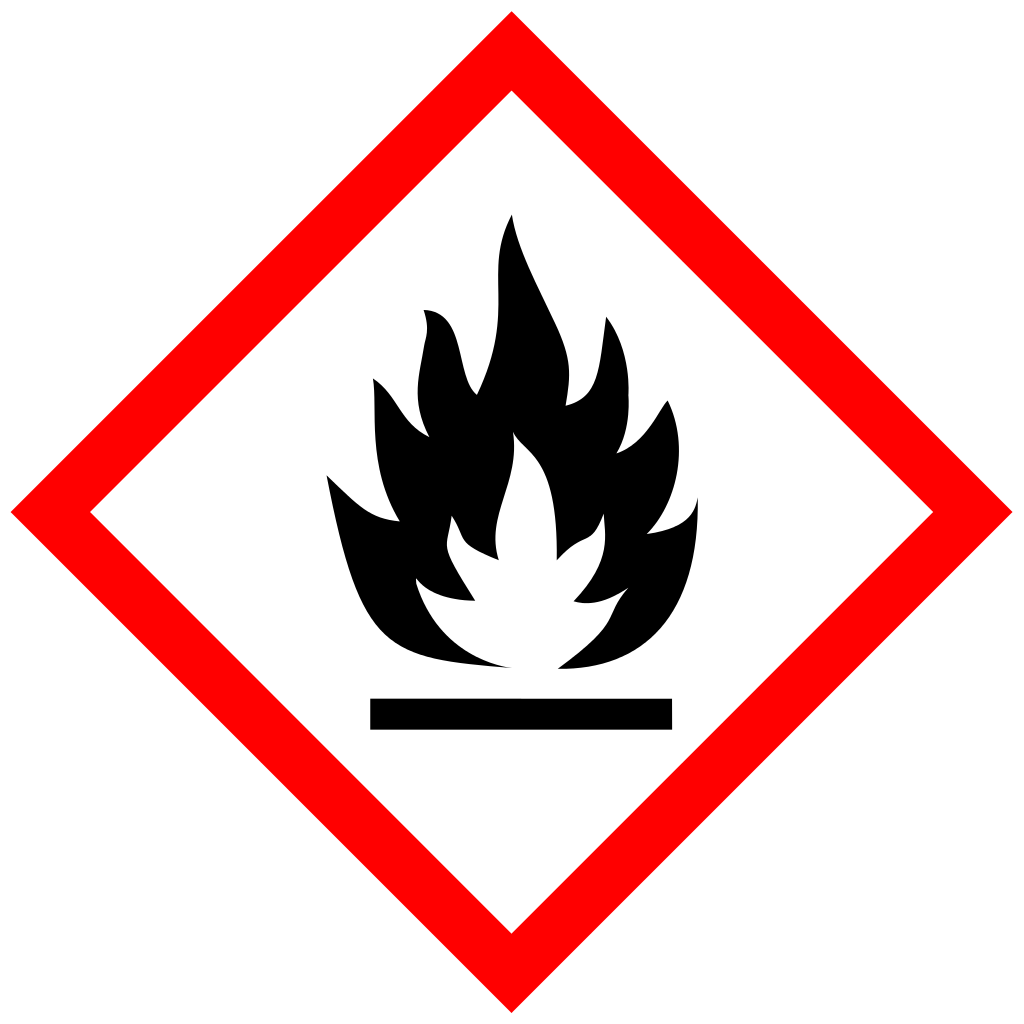
\includegraphics[height=0.1\textheight]{Bilder/Optische_Wellenleiter_Die_Polymer_Optische_Faser/Material_Polycarbonat/flamme.png}
                \caption[entzündlicher Stoff \newline \url{https://de.wikipedia.org/wiki/Datei:GHS-pictogram-flamme.svg} (zuletzt aufgerufen am 11.10.2015)]{entzündlicher Stoff}
                \label{fig:flamme}
            \end{center}
        \end{minipage}
        \hspace{0.025\textwidth}
        \begin{minipage}[t]{0.25\textwidth}
            \begin{center}
                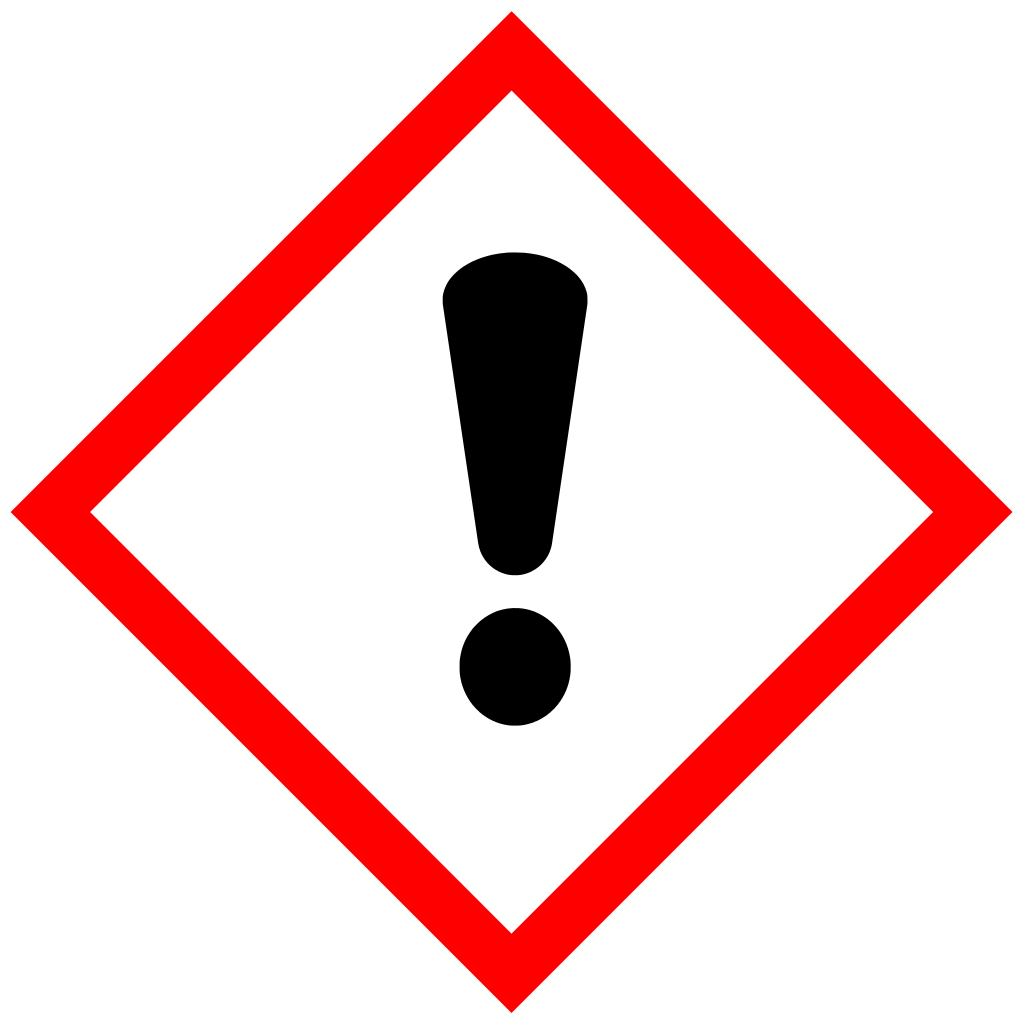
\includegraphics[height=0.1\textheight]{Bilder/Optische_Wellenleiter_Die_Polymer_Optische_Faser/Material_Polycarbonat/ausrufezeichnen.png}
                \caption[reizender Stoff \newline \url{https://de.wikipedia.org/wiki/Datei:GHS-pictogram-exclam.svg} (zuletzt aufgerufen am 11.10.2015)]{reizender Stoff}
                \label{fig:ausrufezeichen}
            \end{center}
        \end{minipage}
        \hspace{0.025\textwidth}
        \begin{minipage}[t]{0.25\textwidth}
            \begin{center}
                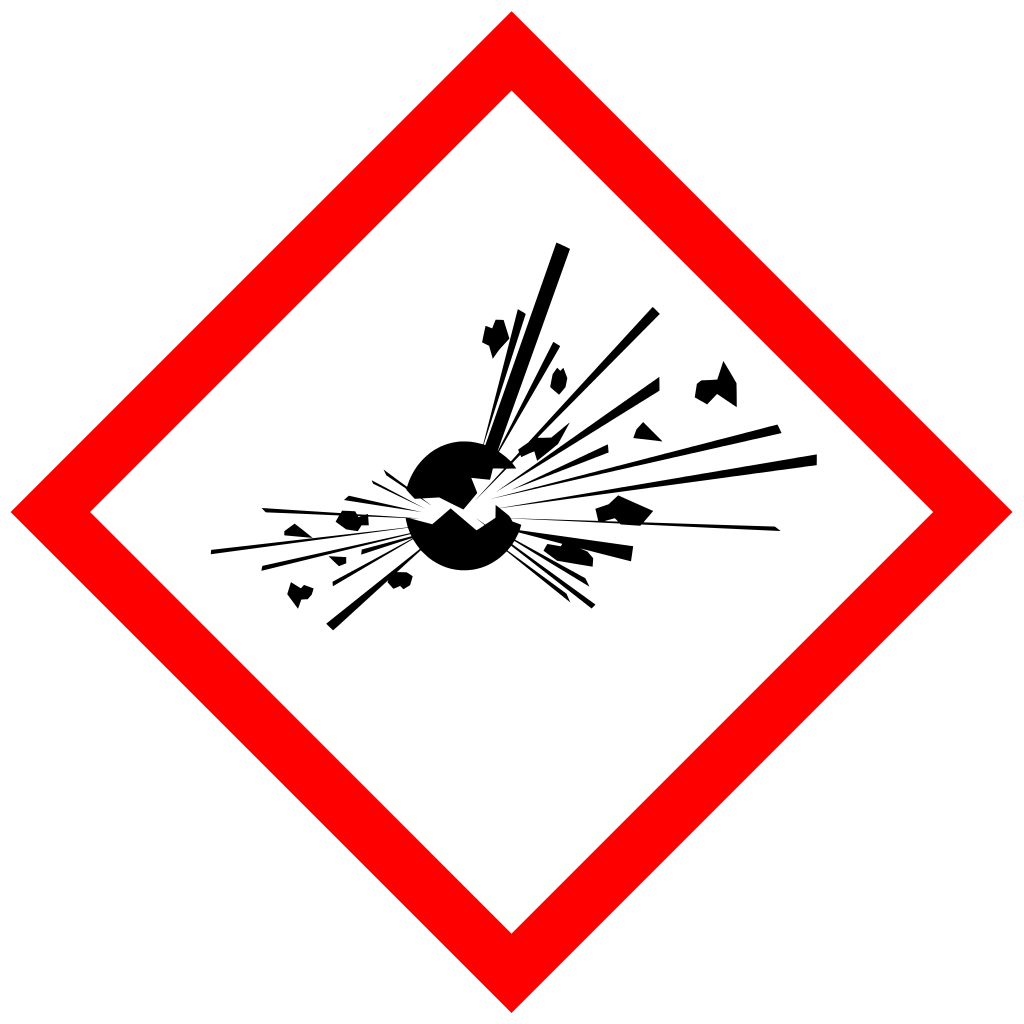
\includegraphics[height=0.1\textheight]{Bilder/Optische_Wellenleiter_Die_Polymer_Optische_Faser/Material_Polycarbonat/bombe.png}
                \caption[explosiver Stoff \newline \url{https://de.wikipedia.org/wiki/Datei:GHS-pictogram-explos.svg} (zuletzt aufgerufen am 11.10.2015)]{explosiver Stoff}
                \label{fig:bombe}
            \end{center}
        \end{minipage}
    \end{center}
\end{figure}

Schutzvorkehrungen:
\begin{itemize}
    \item Abzug, Schutzkleidung, Handschuhe, Schutzbrille
\end{itemize}

Versuchsablauf:
\begin{enumerate*}
    \item Das Wasserbad wird unter dem Abzug auf ca. 60°C erhitzt.
    \item In die Reagenzgläser werden 5 ml MMA mit 50 mg BPO / AIBN vermischt und in das Wasserbad gestellt (siehe \autoref{fig:mmawasserbad}).
    \item Sobald der Inhalt der Reagenzgläser zäh flüssig ist kann es aus dem Wasserbad genommen werden.
    \item Sobald die Polymerisation abgeschlossen ist, wird das Reagenzglas zerschlagen und des PMMA kann entnommen werden.
\end{enumerate*}

\begin{figure}[h]
    \begin{center}
        \begin{minipage}[t]{0.4\textwidth}
            \begin{center}
                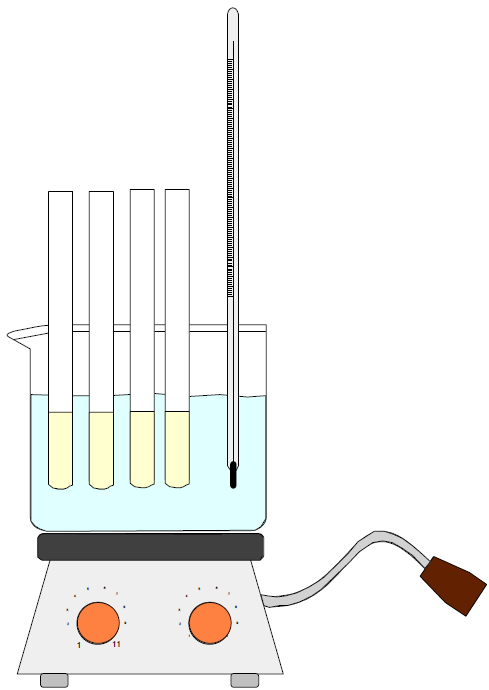
\includegraphics[height=0.1\textheight]{Bilder/Optische_Wellenleiter_Die_Polymer_Optische_Faser/Material_Polycarbonat/mmawasserbad.png}
                \caption[Versuchsaufbau]{Versuchsaufbau}
                \label{fig:mmawasserbad}
            \end{center}
        \end{minipage}
        \hspace{0.025\textwidth}
        \begin{minipage}[t]{0.4\textwidth}
            \begin{center}
                \includegraphics[height=0.1\textheight]{Bilder/Optische_Wellenleiter_Die_Polymer_Optische_Faser/Material_Polycarbonat/pmmastuecke.png}
                \caption[PMMA]{PMMA}
                \label{fig:cdquillt}
            \end{center}
        \end{minipage}
    \end{center}
\end{figure}

Ergebnis:
Die entstandenen PMMA-Stücke haben eine geringe Qualität, da Luftblasen in dem Kunststoff eingeschlossen sind und und sich im
